%%%%%%%%%%%%%%%%%%%%%%%%%%%%%%%%%%%%%%%%%%%%%%%%%%%%
\section{Informed Plan Selection}\label{sec:coverage}
%%%%%%%%%%%%%%%%%%%%%%%%%%%%%%%%%%%%%%%%%%%%%%%%%%%%

Our new approach relies on the idea that confidence in a plan's
\dt\ increases as more of the possible choices below the plan
in the goal-plan structure are explored.

So, with each plan in the goal-plan tree hierarchy, we identify its set of
potential \textit{choices} as the set of all potential execution paths
\textit{below} the plan in the hierarchy. This can easily be computed offline.
% %
Intuitively, a plan's \dt\ is more \textit{informed} for a world state if it is
based on a larger number of choices having been explored in that state. We say
that a plan has a higher degree of \emph{coverage} as more of its underlying
choices are explored and accounted for in the corresponding \dt. Technically,
given a \dt\ $T$ for a certain plan, we define its coverage for the world state
$w$ as $c_T(w) \in [0,\ldots,1]$.
% %
Initially, when the plan has not yet been executed in a world $w$, its coverage
in such state is $c_T(w) = 0$ and the agent has no basis for confidence in the
likelihood of success estimated by $T$ for $w$.
% %
As the different ways of executing the plan in the world state $w$ are explored,
the value of $c_T(w)$ approaches $1$. When all choices have been tried,
$c_T(w)=1$ and the agent may rely fully on the \dt\ estimation of success.
% %
In this way, coverage provides a confidence measure for the \dt\ classification.


We then construct a probabilistic plan selection function that includes the
coverage-based confidence measure.
% %
Formally, we define the plan selection weight $\Omega'(w)$ as a function of the
\dt\ determined success expectation $p_T(w)$ and the degree of coverage $c_T(w)$:
\begin{equation*}\label{eqn:coverage}   
\Omega'_T(w) = 0.5 + \left[  c_T(w) *  \left( p_T(w) - 0.5 \right)  \right].
\end{equation*}
	
	
Initially the selection weight of the plan for a previously unseen world state $w$ takes the default value of $0.5$.
% %
Over time, as the various execution paths below the plan are tried in $w$, its coverage increases 
and the selection weight approaches the true value estimated by the plan's \dt.


%Regarding how the coverage degree is calculated at every point, we should make
%the following two observations.
% %
Each time a plan execution result is recorded, the coverage
$c_T(w)$ for a world $w$ is calculated and stored.
% %
It requires, in principle, $\tau \times |S|$ \emph{unique} executions of
a plan for it to reach \emph{full} coverage, where $\tau$ is the total number of
choices below the plan and $|S|$ is the number of possible worlds. Practically,
however, it takes significantly less since choices below a plan are effectively
an AND/OR tree, and each time an AND node fails, the subsequent
nodes are not tried and are counted as covered for the world in question.
% %
Also, a plan is generally not executed in every world state, so in
practice it will only need to be assessed in the subset of the world
states that is relevant to it.






We are now ready to revisit the two learning approaches \CL\ and \BUL\
from the previous section, but this time using the modified selection weighting
based on coverage.
% %
We will refer to the new approaches as \CLSELB\ and \BULSELB, respectively.
% %
Similarly, $\CLSELA$ and $\BULSELA$ correspond to the approaches using the
\emph{original} selection weighting that only uses its \dt\ success
expectation, that is, $\Omega_T(w) = p_T(w)$.


Our first observation is that the $\BULSELA$ and $\BULSELB$ approaches show
similar performance.
% %
This is not surprising, as the stability test performed by these agents at each
plan node inherently results in close to full coverage. Indeed, for a plan to
become ``stable,'' the agent needs to (substantially) explore all possible  ways
of executing it. The stability check, then, effectively reduces $\Omega'_T(w)$ to
$\Omega_T(w)$.
% %
So, for simplicity, we shall not give a further account of the $\BULSELB$
approach in this section.



We now focus on the \CL\ approach.
% %
For the \CL-favouring structure $\T_1$, we find that the performance of $\CLSELB$ matches that
of $\CLSELA$ reported earlier in Figure~\ref{fig:T1_result}.
% %
Similarly, for the balanced structure $\T_3$ where previously both \CL\ and
\BUL\ performed equally well, the performance of $\CLSELB$
was the same as that reported for $\CLSELA$ earlier in Figure~\ref{fig:T3_result}.
% %
Thus, for the cases where $\CLSELA$ was performing reasonably well, the new $\CLSELA$ approach maintains comparable performance.

\begin{figure}[t]
\begin{center}
%!TEX root = ../dsingh-aamas10-poster.tex
\begin{tikzpicture}[x= 0.00533cm,y=9cm]
	\definecolor{darkblue}{rgb}{0.1,0.1,0.5}
	\definecolor{darkred}{rgb}{0.8,0.0,0.1}
    % Draw the axes and grid lines
    \draw[-] (0,0) -- (0,1) -- (3000,1) -- (3000,0) -- cycle; 
    \draw[-,thin, dotted, ystep=0.2, xstep=3000] (0,0) grid (3000,1);
    \foreach \x in {500, 1500, 2500}  \draw [-,xshift=0](\x,4pt) -- (\x,-1pt);
    \foreach \y in {0.0,0.2,0.4,0.6,0.8,1.0}  \draw [-,yshift=0](4pt,\y) -- (-1pt,\y);
    \foreach \x/\xtext in {500/500, 1500/1500, 2500/2500} \node at (\x,0) [below] {\xtext};
    \foreach \y/\ytext in {0.0,0.2,0.4,0.6,0.8,1.0}  \node at (0,\y) [left] {\ytext};
    \node at (0,1.15) {Success};
    \node at (2500,0.1) {Iterations};
    \draw[-,darkred] plot[mark=x,mark size=10,mark options={color=darkred}] 
			file {figs/data/test05v3gm.CC.tikzdata};
    \draw[-,thin, densely dashed,black] plot[mark=x,mark size=10,mark options={color=black}] 
			file {figs/data/test05v3gm.CP.tikzdata};
    \draw[-,darkblue] plot[mark=o,mark size=6,mark options={color=darkblue}] 
			file {figs/data/test05v3gm.SP.tikzdata};
    % Also draw the expected convergence: 0.9^8 actions=0.43046
    \draw[dashed,-,yshift=0](0,0.43046) -- (3000,0.43046);
	\node at (3450,0.5) {$\mathcal{T}2$};

\end{tikzpicture}

\caption{Performance of $\CLSELB$ (solid crosses) in structure $\T_2$ compared against
the earlier results for $\CLSELA$ and $\BULSELA$ (both in dotted grey).}
\label{fig:T2_result2}
\end{center}
\end{figure}

The benefit of the coverage-based approach is apparent, though, when one
considers the goal-plan structure $\T_2$ in which the $\CLSELA$ performed
poorly (cf. Figure \ref{fig:T2_result}).
% %
Here, the $\CLSELB$ scheme showed a dramatic improvement over $\CLSELA$. Figure
\ref{fig:T2_result2} shows this change with the results for the new approach to
plan selection $\CLSELB$ superimposed over the original results
from Figure \ref{fig:T2_result}.
% %
The reason why the new plan selection mechanism improves the \CL\ learning scheme
is that even though the success estimation $p_T(w)$ for a given plan $P_i$ would
still be low initially (remember that \CL, in contrast with \BUL, would record
all initial failure outcomes for $P_i$), the agent would not be very confident in
such estimation until the plan's coverage increases; therefore the
selection weight $\Omega'_T(w)$ will initially bias towards the default weight of
$0.5$. In other words, the false negative outcomes collected by the agent for
plan $P_i$ would not be considered so seriously due to low plan coverage. As full
coverage is approached, one would expect the agent to have discovered the success
execution encoded in $P_i$.


Even more interesting is the the impact of the new plan selection mechanism on
agents that work with an applicability threshold, i.e., agents that may not
select plans that are deemed unlikely to succeed.
% %%%
Here, the original $\CLSELA$ approach completely fails, as it collects many
negative experiences early on, quickly causing plans' success expectation to fall
below the selection threshold. For $\CLSELB$, even if a plan is deemed with very
low expectation of success, its selection weight would be biased towards the
default value of $0.5$ if it has not been substantially ``covered.''
% %
Hence, provided that the applicability threshold is lower than the default plan
selection weight, then $\CLSELB$ is indeed able to find the solution(s).
% %
Figure~\ref{fig:performance-applicability} shows the $\CLSELB$ performance in
goal-plan structure $\T_2$ for an applicability threshold of $0.2$.


\begin{figure}[t]
   \centering
   %!TEX root = ../dsingh-aamas10.tex
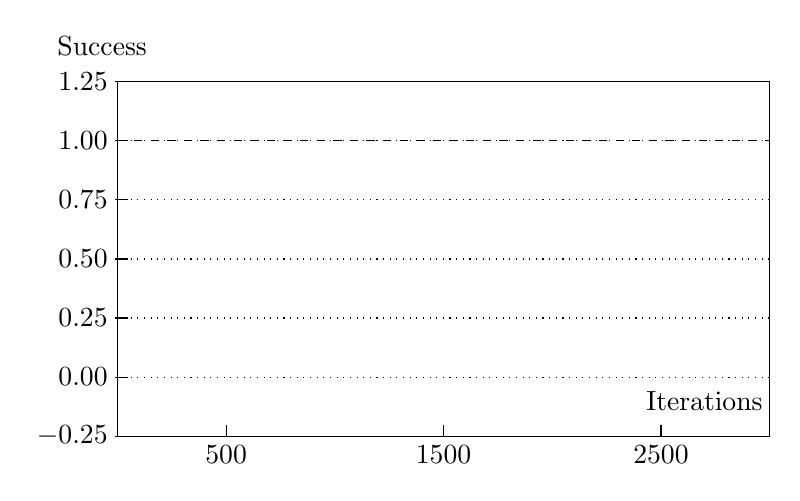
\begin{tikzpicture}[x=0.00276cm,y=3cm]
    % Draw the axes and grid lines
    \draw[-] (0,-0.25) -- (0,1.25) -- (3000,1.25) -- (3000,-0.25) -- cycle; 
    \draw[-,thin, dotted, ystep=0.25, xstep=3000] (0,-0.25) grid (3000,1.25);
    \foreach \x in {500, 1500, 2500}  \draw [-,xshift=0,yshift=-0.25](\x,-0.20) -- (\x,-0.25);
    \foreach \y in {-0.25,0.00,0.25,0.50,0.75,1.00,1.25}  \draw [-,yshift=0](4pt,\y) -- (-1pt,\y);
    \foreach \x/\xtext in {500/500, 1500/1500, 2500/2500} \node at (\x,-0.25) [below] {$\xtext$};
    \foreach \y/\ytext in {-0.25,0.00,0.25,0.50,0.75,1.00,1.25}  \node at (0,\y) [left] {$\ytext$};
    \node at (-70,1.4) {Success};
    \node at (2700,-0.1) {Iterations};
    \draw[-,red] plot[mark=x,mark size=4,mark options={color=red}] 
			file {figs/data/test05v3gmt.CP.tikzdata};
    \draw[-,blue] plot[mark=o,mark size=2,mark options={color=blue}] 
			file {figs/data/test05v3gmt.SP.tikzdata};
    % Also draw the expected convergence: 0.9^8 actions=0.43046
    \draw[dashed,-,yshift=0](0,1.0) -- (3000,1.0);

\end{tikzpicture}

   \caption{Performance of $\CLSELB$ (solid crosses) compared against $\CLSELA$ and $\BULSELA$ (both in dotted grey) in structure $\T_2$ using an applicability threshold of $0.2$.}
   \label{fig:performance-applicability}
\end{figure}


The above results show that the coverage-based confidence weighting can improve
the performance of the \CL\ approach in those cases where it performed poorly due
to false negative experiences, i.e., failure runs for a plan that includes
successful executions.
% %
Furthermore, coverage provides a flexible mechanism for tuning agent behaviour
depending on application characteristics. Consider equation $\Omega'_T(w)$ with
the coverage term modified to $c_T(w)^{1/\alpha}$, with parameter $\alpha \in
[0,\ldots,\infty)$.
% %
Interestingly, as $\alpha \approx 0$, $\CLSELB$ will behave more like $\BULSELA$:
$c_T(w)^{1/\alpha}$ transitions directly from $0$ to $1$ when $c_T(w)$ reaches
$1$ (and remains zero otherwise).
% %
On other hand, when $\alpha \approx \infty$, $\CLSELB$ will behave more like the
$\CLSELA$: $c_T(w)^{1/\alpha}$ transitions from $0$ to $1$ faster and $\Omega'(w)
\approx p_T(w)$. With $\alpha=1$ we get our initial equation.
% %
It follows then that \CLSELB\ provides a \emph{middle ground} between
the \CLSELA\ and \BULSELA\ schemes.


Finally, we note that coverage-based selection weights encourage the agent to
explore all available options. This further ensures that all solutions are
systematically found, allowing the agent to decide which solution is optimal
faster. For some domains this may be an important feature.

